%\documentclass[11pt,a4paper]{memoir}
\documentclass[11pt,a4paper]{article}
%\documentclass[11pt,a4paper]{scrartcl}
\usepackage[table]{xcolor}
%\usepackage{colortbl}
\usepackage{pgfplots}
\usepackage[british,UKenglish,USenglish,english,american]{babel}
%\usepackage[a4paper, total={16cm, 23cm}]{geometry}
\usepackage[tmargin = 1.25in,bmargin = 1.25in,lmargin = 1in,rmargin = 1in]{geometry}
\usepackage{tikz}
\usepackage{graphicx}
\usepackage{chemmacros}
\usepackage{chemfig}
%\usepackage{ghsystem}
\usechemmodule{redox}
%\usepackage{chemnum}
%\usepackage{bohr}
%\usepackage{elements}
%\usepackage{endiagram}
%\usepackage{modiagram}
%\usepackage{chemgreek}
\usepackage{mhchem}
\usepackage{enumitem}
\usepackage{makeidx}
\usepackage{epstopdf}
\usepackage{amssymb}
\usepackage{mathrsfs}
%\usepackage{minted}
\usepackage{amsmath}
\usepackage{enumitem}
\usepackage[english]{varioref}
\usepackage[english]{babel}
\usepackage{lipsum}
\usepackage{fancyhdr}
\pagestyle{fancy} 
\usepackage{float}
\usepackage{empheq}
\usepackage[framemethod=tikz]{mdframed}
\usepackage{epstopdf}
\numberwithin{equation}{section}
\usepackage{eso-pic}
\usepackage{calc}
\usepackage{nccmath}
\usepackage{caption}
\usepackage{subcaption}
\usepackage{gensymb}
\usepackage{amsfonts,amsthm,epsfig,epstopdf,titling,url,array}
\usepackage{siunitx}
\usepackage{xcolor}
\usepackage{multicol}
\usepackage{boondox-cal}
%\usepackage{paralist}




\DeclareSIUnit\atm{atm}

\fancypagestyle{firstpage}{
	\rhead{\begin{picture}(0,0) \put(-30,0){
\includegraphics[width=1cm]{figures/MCI_4C_bw.eps}} \end{picture}}
}
\fancyhead[L]{\slshape\nouppercase{\leftmark}}
\chead{}
\rhead{\begin{picture}(0,0) \put(-30,0){
\includegraphics[width=1cm]{figures/MCI_4C_bw.eps}} \end{picture}}
\lfoot{\textit{}}
\cfoot{-\ \thepage\ -}
\rfoot{\textit{}}
\renewcommand{\headrulewidth}{0.4pt}
\renewcommand{\footrulewidth}{0.4pt}
\newcommand{\abs}[1]{\left|#1\right|}
\definecolor{mycolor1}{rgb}{0.95, 0.95, 0.95}
\definecolor{mycolor2}{rgb}{0.95, 0.95, 0.95}
\definecolor{tableShade}{gray}{0.9}
\newcommand{\sign}{\text{sign}}
\newcommand{\centered}[1]{\begin{tabular}{@{}l@{}} #1 \end{tabular}}
\theoremstyle{it}
\newtheorem{defn}{Definition}[section]
\newtheorem{thm}{Theorem}[section]
\theoremstyle{definition}
\newtheorem{example}{Example}[section]

\newenvironment{myitemize_1}
{ \begin{itemize}[topsep=0pt]
		\setlength{\topsep}{2pt}		
		\setlength{\itemsep}{2pt}
		\setlength{\parskip}{2pt}
		\setlength{\parsep}{2pt}     }
	{ \end{itemize}                  }


\newmdenv[innerlinewidth=0.5pt, roundcorner=4pt,backgroundcolor=mycolor2, linecolor=mycolor1,innerleftmargin=6pt,
innerrightmargin=6pt,innertopmargin=6pt,innerbottommargin=6pt]{mybox}

\title{\textbf{PEM Fuel Cell digital twin model description}}
\author{\textbf{DTL}}

\begin{document}
	\thispagestyle{firstpage}
	\begin{mybox}
		\maketitle
		\vspace{125mm}
	\end{mybox}
	\newpage
	\tableofcontents
	\listoffigures	
	\listoftables
	\newpage

{In this document we describe the proton exchange membrane (PEM) fuel-cell (PEMFC) represented in the Digital Twin Library. The principle of function is based on Nernst equation and it considers the electrochemical reaction between two elements: Hydrogenium and Oxygenium. The model consider the case of a Fuel-Cell Stack which represent a matrix of single elementary cells connect in series and parallel.}

\section{Description}
Fuel cells are static energy conversion devices that convert the chemical energy of fuel directly into dc electrical energy. The physical structure of a fuel cell consist of two porous electrodes (anode and cathode) and an electrolyte layer in the middle. Figure~\ref{pem_fc_intro_2} shows the basic working of a fuel cell with positive ion flow through the electrolyte, which is based on electrochemical principles, like Gibbs free energy (for completeness see §\ref{fundamental}).
\begin{figure}[H]
	\centering
	\includegraphics[width = 0.5\textwidth, width = 250pt, angle = 0, keepaspectratio]{figures/pem_fuel_cell/basic_working.eps}
	\captionsetup{width=0.5\textwidth}		
	\caption{The basic working of fuel cell with proton flow through the electrolyte.}
	\label{pem_fc_intro_2}
\end{figure}
Consider the following reactions, see also Figure~\ref{pem_fc_intro_0}, at anode
\begin{center}
	\ce{2H_2 -> 4H^{+} + 4e^{-}}
\end{center}
and at cathode:
\begin{center}
\ce{O_2 + 4e^{-} + 4H^{+} -> 2H2O_$\mathcal{(g)}$}
\end{center}


\begin{figure}[H]
	\centering
	\includegraphics[width = 0.5\textwidth, width = 320pt, angle = 0, keepaspectratio]{figures/pem_fuel_cell/pem_fuel_cell_0.eps}
	\captionsetup{width=0.5\textwidth}		
	\caption{Schematic diagram and chemical reaction of PEMFC.}
	\label{pem_fc_intro_0}
\end{figure}

\section{Equations}
The partial pressure, transport and electrochemical equations for a single cell based on PEM are reported as follows\footnote{where with the symbol $p^*$ the partial pressure is denoted, as follows \begin{equation}\label{ele_chem_28}
		p^*=\frac{p}{p^\circ}\qquad p^\circ=\SI{100}{\kilo\pascal}
\end{equation}}
\begin{equation}\label{cell_eq}
	\left\lbrace \begin{aligned}
		&	p^\circ\frac{V_a}{RT}\frac{dp_{H_2}^*}{dt} = M_{H_2,in} - M_{H_2,out} - \frac{i}{2F} = M_{H_2,net} - \frac{i}{2F} \\[8pt]
		&	p^\circ\frac{V_c}{RT}\frac{dp_{O_2}^*}{dt} = M_{O_2,in} - M_{O_2,out} - \frac{i}{4F} = M_{O_2,net} - \frac{i}{4F} \\[8pt]
		&	\tau_{a}\frac{dM_{H_2,net}}{dt} = \frac{i}{2F} - M_{H_2,net} \\[8pt]
		&	\tau_{c}\frac{dM_{O_2,net}}{dt} = \frac{i}{4F} - M_{O_2,net} \\[8pt]
		&	E_{cell} = E_{0,cell} + \frac{RT}{2F}\log\Bigg[{p_{H_2}^*\cdot\Big(p_{O_2}^*\Big)^{\frac{1}{2}}}\Bigg] \\[8pt]
		&	E_{0,cell} = \frac{\Delta G}{n_eF} - k_E(T-298)
	\end{aligned}\right. 
\end{equation}
where $V_a$ ($V_c$) is the volume of the anode (cathode) channel $\Big[\SI{}{\cubic\meter}\Big]$; $M_{H_2}=H_2$, mole flow rate $\Big[\SI{}{\mole\per\second}\Big]$; $i$ the fuel cell current $\Big[\SI{}{\ampere}\Big]$; $M_{O_2}=O_2$, mole flow rate $\Big[\SI{}{\mole\per\second}\Big]$; subscripts $\Big(_{in}\Big)$, $\Big(_{out}\Big)$ and $\Big(_{net}\Big)$ denote the values related to input, output, and net. $T=T(t)$ is the cell temperature. 
\begin{figure}[H]
	\centering
	\includegraphics[width = 0.5\textwidth, width = 250pt, angle = 0, keepaspectratio]{figures/pem_fuel_cell/pem_fuel_cell_1.eps}
	\captionsetup{width=0.5\textwidth}		
	\caption{Schematic diagram of a PEM fuel cell and voltage drop across it.}
	\label{pem_fc_intro_1}
\end{figure}

\begin{figure}[H]
	\centering
	\includegraphics[width = 0.5\textwidth, width = 250pt, angle = 0, keepaspectratio]{figures/pem_fuel_cell/pemfc_eq_circuit_1.eps}
	\captionsetup{width=0.5\textwidth}		
	\caption{Equivalent circuit of the double-layer charging effect inside a PEMFC.}
	\label{pem_fc_eq_circuit_intro_1}
\end{figure}

As shown in Figure~\ref{pem_fc_intro_1} under normal operating conditions, the fuel cell output voltage is less than $E_{cell}$ due to the fuel cell activation loss, ohmic voltage drop, and concentration voltage drop across the fuel cell. Therefore,
\begin{equation}
	V_{cell} = E_{cell} - V_{act,cell} - V_{ohm,cell}-V_{conc,cell}
\end{equation}
where $V_{cell}$, $V_{act,cell}$, $V_{ohm,cell}$, and $V_{conc,cell}$ are the cell output voltage, activation voltage drop, ohmic voltage drop, and concentration voltage drop, respectively.

The overall results applied to the single cell can be used in lumped way when a stack of $N_{cells}$ are assembled together. 

In the following a $N_{cells}$ stack is considered and additional voltage drops due to the current load effects are is taken into account as well as the effects of the double layer capacitance created by the membrane
\begin{equation}\label{voltage_drop_equations}
	\left\lbrace \begin{aligned}
		&	V_{ohm} = V_{ohm,a} + V_{ohm,membrane} + V_{ohm,c} = IR_{ohm} \\[8pt]
		&	R_{ohm} = R_{ohm,0} + k_{RI}I - k_{RT}T \\[8pt]
		&	R_{conc}=\frac{V_{conc}}{I}=-\frac{RT}{zFI}\log\Big(1-\frac{I}{I_{\text{limit}}}\Big) \\[8pt]
		&	V_{C}=\Big(I-C\frac{dV_C}{dt}\Big)\big(R_{act}+R_{conc}\big) \\[8pt]
		&	V_{out} = N_{cells}E_{cell} = E - V_{act1} - V_C - V_{ohm}
	\end{aligned}\right. 
\end{equation}
where $V_{out}$ is the output voltage of the PEM fuel cell stack.

\section{Fundamental of PEM fuel cell}\label{fundamental}
A fuel cell is a device in which a fuel is oxidized electrochemically to produce electric power. It has some characteristics of a battery, in fact, it consists of two electrodes separated by an electrolyte. However, the reactants are not stored in the cell but are fed to it continuously, and the products of reaction are continuously withdrawn. The fuel cell is thus not given an initial electric charge, and in operation it does not lose electric charge. It operates as a continuous-flow system as long as fuel and oxygen are supplied, and it produces a steady electric current. Compared to the conventional process of burning a fuel and extracting mechanical work via a heat engine to power a generator, fuel cells provide a more efficient means of converting the chemical energy available by oxidation of fuel into electrical energy.

In a fuel cell, the fuel, e.g. hydrogen, methane, butane, methanol, etc., makes intimate contact with an anode or fuel electrode, and oxygen (usually in air)  makes intimate contact with a cathode or oxygen electrode. Half-cell reactions occur at each electrode, and their sum is the overall reaction. Several types of fuel cell exist, each characterized by a particular type of electrolyte.

Cells operating with hydrogen as fuel is shown in Figure~\ref{pem_fc_2}.
\begin{figure}[H]
	\centering
	\begin{subfigure}{.5\textwidth}
		\centering
		\includegraphics[width = 0.5\textwidth, width = 220pt, keepaspectratio]{figures/pem_fuel_cell/pem_fuel_cell_2.eps}
		\captionsetup{width=0.5\textwidth}		
		\caption{Acid Electrolyte.}
		\label{}
	\end{subfigure}%
	\begin{subfigure}{.5\textwidth}
		\centering
		\includegraphics[width = 0.5\textwidth, width = 220pt, keepaspectratio]{figures/pem_fuel_cell/pem_fuel_cell_3.eps}
		\captionsetup{width=0.5\textwidth}		
		\caption{Alkaline Electrolyte.}
		\label{}
	\end{subfigure}
	\caption{Schematic diagram of different fuel cells}
	\label{pem_fc_2}
\end{figure}
When the electrolyte is acid, the half-cell reaction occurring at the hydrogen electrode (anode) is:
\begin{center}
	\ce{H_2 -> 2H^{+} + 2e^{-}}
\end{center}
and that at the oxygen electrode (cathode) is
\begin{center}
	\ce{\frac{1}{2} O_2 + 2e^{-} + 2H^{+} -> H2O_$\mathcal{(g)}$}
\end{center}
When the electrolyte is alkaline, the half-cell reaction at the anode is
\begin{center}
	\ce{H_2 +2HO^{-} -> 2H2O_$\mathcal{(g)}$ + 2e^{-}}
\end{center}
and at cathode:
\begin{center}
	\ce{\frac{1}{2} O_2 + 2e^{-} + H2O_$\mathcal{(g)}$ -> 2OH^{-}}
\end{center}

This of course is the \textit{combustion reaction} of hydrogen, but combustion in the conventional sense of burning does not occur in the cell.
In both cells electrons with negative charge (\ce{e^{-}}) are released at the anode, produce an electrical current in an external circuit, and are taken up by the reaction occurring at the cathode. The electrolyte does not allow the passage of electrons, but it provides a path migration of an ion from one electrode to the other. With an acid electrolyte, protons (\ce{H^{+}}) migrate from anode to cathode, whereas with an alkaline electrolyte hydroxyl ions (\ch{OH^{-}}) migrate from cathode to anode.



\subsection{Background on electrochemical process}
\noindent\textbf{According to the first law of thermodynamics}, the energy of a system (considered in the form of heat or work) is conserved, meaning that the energy can be neither created nor destroyed, but it can be converter from one type to another. The change in the system energy ($dE$) is contributed by the heat entering the system ($dQ$) and the work done by the system ($dW$).
\begin{equation}\label{ele_chem_1}
	dE = dQ-dW
\end{equation}
Note that work in the above equation is defined as work leaving the system. For a \textit{simple system}, the total system energy is equal to the total system internal energy $U$
\begin{equation}\label{ele_chem_2}
	E=U
\end{equation}
In the following we only consider \textit{simple systems}.

For a \textit{control volume}, usually there is an expansion when heat is absorbed by the system at constant pressure. Part of the heat goes into internal energy and causes the system temperature to rise. The rest of the heat is used to expand the system against the pressure ($p$). A property of the system, called \textit{enthalpy} $H$, is used to represent the system state under a given condition. It is the sum of the system internal energy and the product of the system pressure and volume ($V$).
\begin{equation}\label{ele_chem_3}
	H = U + PV
\end{equation}
\textit{Enthalpy} is independent of which way the system reaches its condition, and as a result, the product of the system pressure ($p$) and volume ($V$) is constant. Eq.~\eqref{ele_chem_3} can therefore be written as
\begin{equation}\label{ele_chem_4}
	dH = dQ - dW
\end{equation}
According to Eq.~\eqref{ele_chem_4}, any changes in enthalpy (state) of a system is a result of the difference between the change in the heat entering the system and the work leaving (done by) the system.

According to the first law of thermodynamics, work done by an ideal cyclic thermal process (heat engine), shown in Figure~\ref{thermal_machines} can be defined by
\begin{equation}\label{ele_chem_5}
	W=Q_1-Q_2
\end{equation}
where $W$ is work done by the system to the outside and $Q_1$ and $Q_2$ are the heat entering and leaving the thermal process, respectively.
\begin{figure}[H]
	\centering
	\includegraphics[width = 0.5\textwidth, width = 360pt, angle = 0, keepaspectratio]{figures/pem_fuel_cell/thermal_process.eps}
	\captionsetup{width=0.5\textwidth}		
	\caption{Themal machines.}
	\label{thermal_machines}
\end{figure}
In 1842, French scientist Sadi Carnot presented the relationship between the heat entering and leaving ideal thermal processes and their corresponding temperatures, $T_1$ and $T_2$ as follows
\begin{equation}\label{ele_chem_6}
	\frac{Q_1}{T_1}=\frac{Q_2}{T_2}
\end{equation}
The efficiency of the process then is 
\begin{equation}\label{ele_chem_7}
	\eta_c=\frac{W}{Q_1}=\frac{Q_1-Q_2}{Q_1} = 1-\frac{T_2}{T_1}
\end{equation}
It is clear from Eq.~\eqref{ele_chem_7} that a higher efficienty can be obtained by having a larger difference between $T_2$ and $T_1$.
Another contribution from Carnot is that $Q/T$ can be a state property of the system by showing the equivalence of $Q_1/T_1$ and $Q_2/T_2$. Based on the Carnot's idea, Rudolf Clausius (a Polish scientist, 1822-1888) developed the concept of entropy and presented the second law of thermodynamics. This concept was introduced to indicate the degree of disorder of a system. If the system is undergoing an infinitesimal reversible process with $dQ$ heat entering the system at temperature $T$, then the infinitesimal change in its \textit{entropy} ($S$) is defined as
\begin{equation}\label{ele_chem_8}
	dS=\left. \frac{dQ}{T}\right|_{\text{rev}}
\end{equation}
A reversible process is a process that can be reversed without leaving any traces to its environment. If a cyclic process only consists of reversible processes, then there is no entropy change after a cycle (i.e. $\Delta S=0$). On the contrary, if the cycle contains an irreversible process, then its entropy will change, which corresponds to work done (or received) by the system. Entropy is an important system property, which is very useful in describing a thermodynamic process. The temperature-entropy diagram for a Carnot Cycle is shown in Figure~\ref{temperature_entropy}, where the area $abcd$ represents work done by the system, when the system temperature goes from $T_1$ to $T_2$. Note that $\Delta S=0$ when there is a change in temperature, but no work is done by the system.

The second law of thermodynamics, described by Clausius for a cyclic process, can be written in an infinitesimal form as follows
\begin{equation}\label{ele_chem_9}
	dS\ge\frac{dQ}{T}
\end{equation}
\begin{figure}[H]
	\centering
	\includegraphics[width = 0.5\textwidth, width = 200pt, angle = 0, keepaspectratio]{figures/pem_fuel_cell/temperature_entropy.eps}
	\captionsetup{width=0.5\textwidth}		
	\caption{Temperature-entropy diagram for a Carnot cycle.}
	\label{temperature_entropy}
\end{figure}
In Eq.~\eqref{ele_chem_9}, the equality sign applies to a reversible cyclic process and the inequality sign applies to an irreversible process. That is to say, for any irreversible process, change in work is done in the direction that change in entropy is greater than $dQ/T$. This means that heat cannot be transferred from a low temperature to a higher temperature without a need of work from outside. The second law also reveals that no real heat engine efficiency can reach $100\%$ due to the increase of entropy. For an isolated system, the change of entropy will always be greater than equal to zero.

\textbf{The Gibbs free energy} $G$ is defined as
\begin{equation}\label{ele_chem_10}
	G = H-TS = U + pV - TS
\end{equation}
Differentiating Eq.~\eqref{ele_chem_11} we obtain
\begin{equation}\label{ele_chem_11}
	dG=dH-(TdS+SdT)=dU+pdV+Vdp-(TdS+SdT)
\end{equation}
Chemical reactions proceed toward the direction that minimizes the Gibbs energy. Therefore, $dG$ is negative as a chemical reaction approaches its equilibrium point, and it will be zero at the equilibrium point. According to the first law of thermodynamics, for a \textit{simple system}, Eq.~\eqref{ele_chem_11} can be rewritten as
\begin{equation}\label{ele_chem_12}
	dG=dH-(TdS+SdT)=dQ-dW+pdV+Vdp-(TdS+SdT)
\end{equation}
For systems that are restricted to performing only expansion-type of work, we can write
\begin{equation}\label{ele_chem_13}
	dW=pdV
\end{equation}
Also, the following condition holds if the process is reversible:
\begin{equation}\label{ele_chem_14}
	dQ=TdS
\end{equation}
Substituting Eq.~\eqref{ele_chem_13} and  Eq.~\eqref{ele_chem_14} into  Eq.~\eqref{ele_chem_12} we obtain
\begin{equation}\label{ele_chem_15}
	dG=Vdp-SdT
\end{equation}
Solving the differential equation Eq.~\eqref{ele_chem_15}, Gibbs energy can be obtained at a given temperature ($T$) and under any pressure.
\begin{equation}\label{ele_chem_16}
	G(T)=G^\circ(T)+nRT\log\Big[\frac{p}{p^\circ}\Big]
\end{equation}
In Eq.~\eqref{ele_chem_16} $G^\circ(T)$ is the standard Gibbs energy at temperature $T$ and at $p^\circ=\SI{100}{\kilo\pascal}$.

For an electrochemical reaction, the maximum work (electricity) is determined by the change in the Gibbs energy as the reactions change to products. It can be shown that the maximum electricity production ($W_e$) is equal to the change in the Gibbs energy.
\begin{equation}\label{ele_chem_17}
	W_e=-\Delta G
\end{equation}

In a chemical reaction, the change in enthalpy $\Delta H$ due to the reaction can be written as
\begin{equation}\label{ele_chem_18}
	\Delta H = H_P-H_R=\sum_{P_i}N_{P_i}H_{P_i}-\sum_{R_j}N_{R_j}H_{R_j}
\end{equation}
where $H_{P}$ is the total enthalpy of the products and $H_R$ is the total enthalpy of the reactants. $N_{P_i}$ is the amount of moles of the $i$th species in the products and $N_{R_j}$ is the amount of moles of the $j$th species in the reactants.

Accordingly, $H_{P_i}$ and $H_{R_j}$ are the molar enthalpies of the corresponding species, which can be represented as
\begin{equation}\label{ele_chem_19}
	H_{P_i}=\Big(H_f^\circ+H-H^\circ\Big)_{P_i}
\end{equation}
In Eq.~\eqref{ele_chem_19}, $H_f^\circ$ is the standard molar enthalpy of formation ($\SI{}{\joule\per\mole}$) and ($H-H^\circ$) is the molar enthalpy due to the temperature difference.

The change of entropy due to the reaction can be written as
\begin{equation}\label{ele_chem_20}
	\Delta S = S_P-S_R = \sum_{P_i}N_{P_i}S_{P_i}-\sum_{R_j}N_{R_i}S_{R_i}
\end{equation}
where $S_P$ is the total entropy of the products and $S_R$ is the total entropy of the reactants. $S_{P_i}$ ($S_{R_i}$) is the molar entropy of the corresponding species. The change in Gibbs free energy due to the reaction ($\Delta G$) can than be obtained from Eq.~\eqref{ele_chem_10} as follows
\begin{equation}\label{ele_chem_21}
	\Delta G = \Delta G_P - \Delta G_R=\Delta H-T\Delta S
\end{equation}

Two example reactions are given below for the formation of water, in vapor form and in liquid form, from hydrogen and oxygen, to show how the change in Gibbs energy (or electric energy) in a reaction can be calculated. The enthalpy and entropy values for water, hydrogen and oxygen used in the equations are given in Table~\ref{table_std}. The reactions are assumed to happen under standard conditions ($p=p^\circ$ and $T=\SI{298.15}{\kelvin}$)
\setlength\arrayrulewidth{1pt}
\begin{center}
	\setlength{\extrarowheight}{6pt}
	\begin{tabular}{m{10em}  m{15em}  m{15em}}
		\hline
		 	 & Enthalpy, $H_f\Big[\SI{}{\kilo\joule\per\mole}\Big]$  & Entropy, $S\Big[\SI{}{\joule\per\mole\per\kelvin}\Big]$ \\[6pt]
		\hline
		\ce{H2O_$\mathcal{(g)}$} & -241.8 & 188.7 \\[6pt]
		\ce{H2O_$\mathcal{(l)}$} & -285.8 & 69.9 \\[6pt]
		\ce{H2} & 0 & 130.6 \\[6pt]
		\ce{O2} & 0 & 205 \\[6pt]
		\hline
	\end{tabular}
	\captionsetup{width=0.75\textwidth}		
	\captionof{table}{Standard thermodynamic properties (enthalpy and entropy).}
	\label{table_std}
\end{center}
\begin{equation}\label{ele_chem_22}
	\ce{\frac{1}{2} O_2 + H_2 -> H2O_$\mathcal{(g)}$}
\end{equation}
\begin{equation}\label{ele_chem_23}
	\ce{\frac{1}{2} O_2 + H_2 -> H2O_$\mathcal{(l)}$}
\end{equation}
In the formula shown in \ref{ele_chem_22} and \ref{ele_chem_23}, $\mathcal{(g)}$ and $\mathcal{(l)}$ indicate that the reaction product is in gas or in liquid form, respectively. From Eq.~\eqref{ele_chem_18} and Eq.~\eqref{ele_chem_20}, we have
\begin{equation*}
	\Delta H = H_P-H_R = (-241.8-0.0)=\SI{-241.8}{\kilo\joule\per\mole}
\end{equation*}
\begin{equation*}
	\Delta S = S_P-S_R = (-188.7-130.6-0.5\times205)=\SI{-44.4}{\joule\per\mole\per\kelvin}
\end{equation*}
Therefore, the change in the Gibbs energy of the reaction given in Eq.~\eqref{ele_chem_17} is 
\begin{equation*}
	\Delta G = \Delta H -T\Delta S = -241.8-298\times\Big(-44.4\times10^{-3}\Big)=\SI{-228.57}{\kilo\joule\per\mole}
\end{equation*}
For the reaction given in \ref{ele_chem_23}, we have
\begin{equation*}
	\Delta H = H_P-H_R = (-285.8-0.0)=\SI{-285.8}{\kilo\joule\per\mole}
\end{equation*}
\begin{equation*}
	\Delta S = S_P-S_R = (-69.9-130.6-0.5\times205)=\SI{-163.2}{\joule\per\mole\per\kelvin}
\end{equation*}
Therefore, the change in the Gibbs energy for the formation of water in vapor form (Eq.~\eqref{ele_chem_17}) is
\begin{equation*}
	\Delta G = \Delta H -T\Delta S = -285.8-298\times\Big(-163.2\times10^{-3}\Big)=\SI{-237.16}{\kilo\joule\per\mole}
\end{equation*}
From the above examples, we can see that more work is done if the product (\ch{H_2O}) is in the liquid form.

\subsection{The Nernst equation}
Consider an electrochemical reaction under constant temperature and pressure, where reactants $X$ and $Y$ form products $M$ and $N$ as follows
\begin{equation}\label{ele_chem_24}
	\ce{aX + bY <-> cM + dN}
\end{equation}
where $a$, $b$, $c$ and $d$ are stoichiometric coefficients.

According to Eq.~\eqref{ele_chem_21}, the change in Gibbs energy of the reaction is 
\begin{equation}\label{ele_chem_25}
	\Delta G = \Delta G_P - \Delta G_R= cG_M+dGG_N-aG_X-bG_Y
\end{equation}
The change in the Gibbs energy can also be calculated at different temperature and pressure as follows
\begin{equation}\label{ele_chem_26}
	\Delta G = \Delta G^\circ + RT\log{\Bigg[\frac{\Big(\frac{p_M}{p^\circ}\Big)^c\Big(\frac{p_N}{p^\circ}\Big)^d}{\Big(\frac{p_X}{p^\circ}\Big)^a\Big(\frac{p_Y}{p^\circ}\Big)^b}\Bigg]}
\end{equation}
or 
\begin{equation}\label{ele_chem_27}
	\Delta G = \Delta G^\circ + RT\log{\Bigg[\frac{\Big({p_M^*}\Big)^c\Big({p_N^*}\Big)^d}{\Big({p_X^*}\Big)^a\Big({p_Y^*}\Big)^b}\Bigg]}
\end{equation}
where $\Big(^*\Big)$ mean the \textbf{activity} of the respective reactant and/or product. For the case of gas behaving as \textbf{ideal gas}, it can be shown that 
\begin{equation}\label{ele_chem_28}
	p^*=\frac{p}{p^\circ}\qquad p^\circ=\SI{100}{\kilo\pascal}
\end{equation}
In Eq.~\eqref{ele_chem_27} $\Delta G^\circ$ is given as follows
\begin{equation}\label{ele_chem_29}
	\Delta G^\circ = cG_M^\circ+dG_N^\circ-aG_X^\circ-bG_Y^\circ
\end{equation}

In an electrochemical reaction, work can be considered as the electrical energy delivered by the reaction. The electrochemical work is defined by
\begin{equation}\label{ele_chem_30}
W_e=n_eFE
\end{equation}
where $n_e$ is the number of electrons participating in the reaction, $F$ is the Faraday constant ($\SI{98487}{\coulomb\per\mole}$) and $E$ is the potential difference across the electrodes.

According to Eq.~\eqref{ele_chem_17}, the change in Gibbs energy is the negative value of the work done by the reaction
\begin{equation}\label{ele_chem_31}
	\Delta G = -W_e=-n_eFE
\end{equation}
Under standard condition, Eq.~\eqref{ele_chem_31} can be written as
\begin{equation}\label{ele_chem_32}
	\Delta G^\circ = -W_e^\circ=-n_eFE^\circ
\end{equation}
where $E^\circ$ is the standard reference potential.

Using Eq.~\eqref{ele_chem_31}, the electrode voltage $E$ can be calculated as follows
\begin{equation}\label{ele_chem_33}
	E = -\frac{\Delta G}{n_eF} = -\frac{\Delta G^\circ}{n_eF} - \frac{RT}{2F}\log{\Bigg[\frac{\Big({p_M^*}\Big)^c\Big({p_N^*}\Big)^d}{\Big({p_X^*}\Big)^a\Big({p_Y^*}\Big)^b}\Bigg]}
\end{equation}
Writing Eq.~\eqref{ele_chem_33} in terms of standard reference potential $E^\circ$, the well-known electrochemical formula, the Nernst equation, for calculation of the potential difference between two electrodes can be derived
\begin{equation}\label{ele_chem_34}
	E = E^\circ -  \frac{RT}{2F}\log{\Bigg[\frac{\Big({p_M^*}\Big)^c \Big({p_N^*}\Big)^d}{\Big({p_X^*}\Big)^a\Big({p_Y^*}\Big)^b}\Bigg]} = E^\circ +  \frac{RT}{2F}\log{\Bigg[\frac{\Big({p_X^*}\Big)^a\Big({p_Y^*}\Big)^b}{\Big({p_M^*}\Big)^c\Big({p_N^*}\Big)^d}\Bigg]}
\end{equation}
For fuel-cell with an overall reaction, given by Eq.~\eqref{ele_chem_22} the voltage across the fuel cell electrodes (or the internal potential of the fuel cell) is given by
\begin{equation}\label{ele_chem_35}
	\begin{aligned}
		E = E^\circ + \frac{RT}{2F}\log\Bigg[\frac{{p_{H_2}^*\cdot\Big(p_{O_2}^*\Big)^{\frac{1}{2}}}}{p_{H_2O}^*}\Bigg]
	\end{aligned}
\end{equation}
If the product (\ch{H2O}) is in liquid form, given by the formula~\ref{ele_chem_23}, the the fuel cell internal potential is 
\begin{equation}\label{ele_chem_36}
	\begin{aligned}
		E = E^\circ + \frac{RT}{2F}\log\Bigg[{{p_{H_2}^*\cdot\Big(p_{O_2}^*\Big)^{\frac{1}{2}}}}\Bigg]
	\end{aligned}
\end{equation}







\subsection{Dynamic model of PEM fuel-cell}
For many practical applications the most satisfactory hydrogen/oxygen fuel cell is built around a solid polymer that serves as an acid electrolyte. Because it is very thin and conducts \ch{H^{+}} ions or protons, it is known as a proton-exchange membrane (PEM). Each side of the membrane is bounded to a porous electrode loaded with an electrocatalyst such as finely divided platinum. The porous electrodes provide a very large surface area for reaction and accommodate the diffusion of hydrogen and oxygen into the cell and water liquid out of the cell. Cells can be stacked and connected in series to make very compact units with a desired terminal emf. They typically operate at temperature near $\SI{60}{\celsius}$.

In order to build a dynamic model of a PEM fuel-cell stack, a preliminary mathematical approach is presented. To simplify the analysis, the following assumptions are made.
\begin{enumerate}
	\item One-dimensional treatment.
	\item Ideal and uniformly distributed gases.
	\item Constant pressure in the fuel cell gas flow channels.
	\item The fuel is humidified hydrogen, and the oxidant is humidified air.
	\item On the anode side, the \textbf{water activity vapor pressure}\footnote{$x^*_{H_2O}=\frac{p_{H_2O}^*}{\big(p_{H_2O}^{sat}\big)^*}$ where $p_{H_2O}^*$ is the partial vapor pressure of water in the solution, and $\big(p_{H_2O}^{sat}\big)^*$ is the partial vapor pressure of pure water at the same temperature} is $50\%$ and on the cathode side, $100\%$ of the saturated vapor pressure.
\begin{figure}[H]
	\centering
	\includegraphics[width = 0.5\textwidth, width = 320pt, angle = 0, keepaspectratio]{figures/pem_fuel_cell/pem_fuel_cell_0.eps}
	\captionsetup{width=0.5\textwidth}		
	\caption{Schematic diagram and chemical reaction of PEMFC.}
	\label{pem_fc_0}
\end{figure}
	\item The PEMFC operates under $\SI{100}{\celsius}$ and the reaction product is in liquid phase.
	\item Thermodynamics properties are evaluated at the average stack temperature. Temperature variations across the stack are neglected, and the overall specific heat capacity of the stack is assumed to be constant.
	\item Parameters for individual cells can be lumped together to represent a fuel-cell stack. 
\end{enumerate}
A schematic diagram of a PEM fuel cell and its internal voltage drops are shown in Figure~\ref{pem_fc_1}
In order to calculate the fuel-cell output voltage, the effective partial pressure of \ch{H2} and \ch{O2} need to be determined. In a gas mixture consisting of $n$ specie, the diffusion of component $i$ through the porous electrodes can be described by the Stefan-Maxwell formulation
\begin{equation}\label{eq1}
	\vec{\nabla}x_i = \frac{RT}{p}\sum_{j=1}^{N}\frac{x_iN_j-x_jN_i}{D_{i,j}}
\end{equation}
where $x_i$ ($x_j$) is the mole fraction of the specie $i$ ($j$); $D_{i,j}$ is the diffusivity coefficient between the two species $i$ and $j$ $\Big[\SI{}{\square\meter\per\second}\Big]$; $N_i$ ($N_j$) the superficial gas flow of species $i$ ($j$) in $\Big[\SI{}{\mole\per\square\meter\per\second}\Big]$; $R=\SI{8.3143}{\joule\per\mole\per\kelvin}$ the gas constant; $T\,[K]$ the gas temperature and $p$ the overall pressure of gas mixture in $\Big[\SI{}{\pascal}\Big]$.

The \textbf{the effective partial pressures}\footnote{For gases, the activity is the effective partial pressure, and is usually referred to as \textit{fugacity}.} of hydrogen and oxygen are needed in order to calculate the PEMFC output voltage. At the anode channel, the gas stream is a mixture of \ch{H2} and \ch{H2O_{$\mathcal{(g)}$  }}. The molar flux of water (in gas phase) normal to anode surface can be set to zero, according to hypothesis (1)-(3) given above.

According Eq.~\eqref{eq1}, assuming one dimensional (1-D) transport process along the $x$ axis, as shown in Figure~\ref{pem_fc_1}, the diffusion of water can be simplified as
\begin{equation}\label{eq2}
	\begin{aligned}
		\frac{dx_{H_2O}}{dx}=\frac{RT}{p_a}\Bigg(\frac{x_{H_2O}N_{H_2}-x_{H_2}N_{H_2O}}{D_{H_2O,H_2}}\Bigg)
	\end{aligned}
\end{equation}
where $p_a$ is the overall gas pressure at the anode $\Big[\SI{}{\pascal}\Big]$.

The molar flow of \ch{H2} can be determined by Faraday's Law
\begin{equation}\label{eq3}
	\begin{aligned}
		N_{H_2}=\frac{J}{2F}
	\end{aligned}
\end{equation}
where $F\approx\SI{96485}{\coulomb\per\mole}$ is the Faraday constant and $J$ is a current density $\Big[\SI{}{\ampere\square\meter}\Big]$.

By combining Eq.~\eqref{eq2} and Eq.~\eqref{eq3} and integrating the expression with respect to $x$ from the anode channel to the catalyst surface, it gives
\begin{equation}\label{eq4}
	\begin{aligned}
		x_{H_2O}^* = \Big(x_{H_2O}^{ch}\Big)^*\ \text{exp} \Big(\frac{RTJ\mathcal{l_a}}{2Fp_aD_{H_2O,H_2}}\Big)
	\end{aligned}
\end{equation}
where $\mathcal{l_a}$ is the distance from anode surface to the reaction site $\Big[\SI{}{\meter}\Big]$; superscript $\Big(^*\Big)$, denotes, as already seen, the activity\footnote{The thermodynamic activity of a species is a measure of the \textbf{effective concentration} of a species in a reacting system. By convention, it is a dimensionless quantity. The activity of pure substances in condensed phases (liquid or solid) is taken as unity. Activity depends principally on the temperature, pressure and composition of the system. 
%	In reactions that involve real gases and mixtures, the effective partial pressure of a constituent gas is usually referred to as \textit{fugacity}.
}; superscript $\Big(^{ch}\Big)$ denotes the conditions at the anode or cathode channel.

According to the assumption (4) given above, the fuel consists only of hydrogen and water vapor. That is, at the anode, $x_{H_2O}^*+x_{H_2}^*=\SI{1}{}$. Therefore according to the uniformity of gas distribution along the $x$-axis (assumption - 2), the effective partial pressure of hydrogen \ch{H2} can be written as
\begin{equation}\label{eq5}
	\begin{aligned}
		p_{H_2}^* = \frac{p_{H_2O}^*}{x_{H_2O}^*} \Big(1-x_{H_2O}^*\Big)
	\end{aligned}
\end{equation}
According to assumption (5), $p_{H_2O}^*$ at the anode is $0.5\Big(p_{H_2O}^{sat}\Big)^*$. Therefore, $p_{H_2}^*$ is given as
\begin{equation}\label{eq6}
	\begin{aligned}
		p_{H_2}^* = 0.5\Big(p_{H_2O}^{sat}\Big)^* \Big(\frac{1}{x_{H_2O}^*}-1\Big).
	\end{aligned}
\end{equation}
The gases flowing in the cathode channel are \ch{O2}, \ch{N2}, \ch{H2O} and \ch{CO2}. Using Eq.~\eqref{eq1}, the diffusion of \ch{H2O_{$\mathcal{(g)}$}} at the cathode side can be obtained from 
\begin{equation}\label{eq7}
	\begin{aligned}
		\frac{dx_{H_2O}}{dx}&=\frac{RT}{p_c}\Bigg(\frac{x_{O2}N_{H_2O}-x_{H_2O}N_{O2}}{D_{H_2O,O_2}}\Bigg) \\[6pt]
		&= \frac{RT}{p_c}\Bigg(\frac{-x_{H_2O}N_{O2}}{D_{H_2O,O_2}}\Bigg)
	\end{aligned}
\end{equation}
where $p_c$ is the overall gas pressure at the cathode $\Big[\SI{}{\pascal}\Big]$.

Similar to the analysis for anode, the activity coefficient of \ch{H2O}, \ch{N2} and \ch{CO2} at the cathode catalyst interface can be derived as follows:
\begin{equation}\label{eq8}
	\begin{aligned}
		x_{H_2O}^*=\Big(x_{H_2O}^{ch}\Big)^*\ \text{exp}\Bigg(\frac{RTJ\mathcal{l_c}}{4Fp_cD_{H_2O,O_2}}\Bigg)
	\end{aligned}
\end{equation}
\begin{equation}\label{eq9}
	\begin{aligned}
		x_{N_2}^*=\Big(x_{N_2}^{ch}\Big)^*\ \text{exp}\Bigg(\frac{RTJ\mathcal{l_c}}{4Fp_cD_{N_2,O_2}}\Bigg)
	\end{aligned}
\end{equation}
\begin{equation}\label{eq10}
	\begin{aligned}
		x_{CO_2}^*=\Big(x_{CO_2}^{ch}\Big)^*\ \text{exp}\Bigg(\frac{RTJ\mathcal{l_c}}{4Fp_cD_{CO_2,O_2}}\Bigg)
	\end{aligned}
\end{equation}
where $\mathcal{l_c}$ is the distance from the cathode surface to the reaction site $\Big[\SI{}{\meter}\Big]$; At the cathode the activity coefficient of \ch{O2} is as follows
\begin{equation}\label{eq11}
	\begin{aligned}
		x_{O_2}^*=1-x_{H_2O}^*-x_{N_2}^*-x_{CO_2}^*
	\end{aligned}
\end{equation}
\noindent and the corresponding effective partial pressure of \ch{O2} is 
\begin{equation}\label{eq12}
	\begin{aligned}
		p_{O_2}^* = \frac{p_{H_2O}^*}{x_{H_2O}^*} x_{O2}^*=\frac{p_{H_2O}^*}{x_{H_2O}^*}\Big(1-x_{H_2O}^*-x_{N_2}^*-x_{CO_2}^*\Big).
	\end{aligned}
\end{equation}
According to assumption (5), $p_{H_2O}^*$ at the cathode equals $\Big(p_{H_2O}^{sat}\Big)^*$ and the above equation can be written as
\begin{equation}\label{eq13}
	\begin{aligned}
		p_{O_2}^* = \Big(p_{H_2O}^{sat}\Big)^*\ \Big(\frac{1-x_{N_2}^*-x_{CO_2}^*}{x_{H_2O}^*}-1\Big).
	\end{aligned}
\end{equation}
where $p_{H_2}^*$ and $p_{O_2}^*$ are the partial pressure of the fuel and of the oxidant and will be used in the Nernst equation to find fuel-cell output voltage. 

\subsection{Material conservation}
The instantaneous change in the effective partial pressure of hydrogen and oxygen can be determined through the ideal gas equations as follows
\begin{equation}\label{eq14}
	\begin{aligned}
		p^\circ\frac{V_a}{RT}\frac{dp_{H_2}^*}{dt} = M_{H_2,in} - M_{H_2,out} - \frac{i}{2F} = M_{H_2,net} - \frac{i}{2F}
	\end{aligned}
\end{equation}
\begin{equation}\label{eq15}
	\begin{aligned}
		p^\circ\frac{V_c}{RT}\frac{dp_{O_2}^*}{dt} = M_{O_2,in} - M_{O_2,out} - \frac{i}{4F} = M_{O_2,net} - \frac{i}{4F}
	\end{aligned}
\end{equation}
where $V_a$ ($V_c$) is the volume of the anode (cathode) channel $\Big[\SI{}{\cubic\meter}\Big]$; $M_{H_2}=H_2$, mole flow rate $\Big[\SI{}{\mole\per\second}\Big]$; $i$ the fuel cell current $\Big[\SI{}{\ampere}\Big]$; $M_{O_2}=O_2$, mole flow rate $\Big[\SI{}{\mole\per\second}\Big]$; subscripts $\Big(_{in}\Big)$, $\Big(_{out}\Big)$ and $\Big(_{net}\Big)$ denote the values related to input, output, and net.

At steady state, all partial pressures are considered to be kept constant, that is 
\begin{equation}\label{eq16}
	\begin{aligned}
		\frac{dp_{H_2}^*}{dt} = \frac{dp_{O_2}^*}{dt} = 0
	\end{aligned}
\end{equation}
\begin{figure}[H]
	\centering
	\includegraphics[width = 0.5\textwidth, width = 250pt, angle = 0, keepaspectratio]{figures/pem_fuel_cell/pem_fuel_cell_1.eps}
	\captionsetup{width=0.5\textwidth}		
	\caption{Schematic diagram of a PEM fuel cell and voltage drop across it.}
	\label{pem_fc_1}
\end{figure}
Therefore, the net mole flow rates of \ch{H2} and \ch{O2} at steady state are 
\begin{equation}\label{eq17}
	\begin{aligned}
		M_{H_2,net} = 2M_{O_2,net} = \frac{I}{2F}
	\end{aligned}
\end{equation}
Under transient state, there are delays between the change in load current and the flow of fuel (\ch{H2}) and oxidant \ch{O2}.
Eq.~\eqref{eq14} and Eq.~\eqref{eq14} can be modeled by the following first order differential equations:
\begin{equation}\label{eq18}
	\begin{aligned}
		\tau_{a}\frac{dM_{H_2,net}}{dt} &= \frac{i}{2F} - M_{H_2,net} \\[8pt]
		\tau_{c}\frac{dM_{O_2,net}}{dt} &= \frac{i}{4F} - M_{O_2,net}
	\end{aligned}
\end{equation}
Time constant $\tau_{a}$ and $\tau_{c}$ represent the fuel and oxidant flow delays (in seconds) at the anode and cathode respectively. The dynamic system of Eq.~\eqref{eq18} will be used to determine the output voltage of the PEMFC.

\subsection{PEM-FC output voltage}\label{PEMFC_output_voltage}
According to assumption (5) the corresponding Nernst equation used to calculate the reversible potential is
\begin{equation}\label{eq20}
	\begin{aligned}
		E_{cell} = E_{0,cell} + \frac{RT}{2F}\log\Bigg[{p_{H_2}^*\cdot\Big(p_{O_2}^*\Big)^{\frac{1}{2}}}\Bigg]
	\end{aligned}
\end{equation}
where $E_{0,cell}$ is a function of temperature and can be expressed as follows
\begin{equation}\label{eq21}
	\begin{aligned}
		E_{0,cell} = E_{0,cell}^0 - k_E(T-298)
	\end{aligned}
\end{equation}
where $E_{0,cell}^0$ is the standard reference potential at standard state, $\SI{298}{\kelvin}$ and $\SI{101325}{\pascal}$ pressure.

To simplify the analysis, a voltage $E_{d,cell}$ is considered to be subtracted  from the right side of Eq.~\eqref{eq20} for the overall effect of the fuel and oxidant delay. The steady state value of $E_{d,cell}$ is zero, but it will show the influence of the fuel and oxidant delays on the fuel-cell output voltage during load transient. It can be written as
\begin{equation}\label{eq22}
	\begin{aligned}
		E_{d,cell} = \lambda_e \Big[i(t) - i(t)\circledast\exp(-\frac{t}{\tau_e})\Big]
	\end{aligned}
\end{equation}
where $\circledast$ represent the convolution operator. Converting Eq.~\eqref{eq22} to the Laplace domain, we get
\begin{equation}\label{eq23}
	\begin{aligned}
		E_{d,cell}(s) = \frac{\tau_es}{\tau_es+1} \lambda_eI(s).
	\end{aligned}
\end{equation}
Eq.~\eqref{eq23} is used for developing the model. The internal potential $E_{cell}$ in Eq.~\eqref{eq20} now becomes
\begin{equation}\label{eq24}
	\begin{aligned}
		E_{cell} = E_{0,cell} + \frac{RT}{2F}\log\Bigg[{p_{H_2}^*\cdot\Big(p_{O_2}^*\Big)^{\frac{1}{2}}}\Bigg]-E_{d,cell}
	\end{aligned}
\end{equation}
where $E_{cell}$ calculated from Eq.~\eqref{eq24}, is actually the open-circuit voltage of the fuel-cell. However, under normal operating conditions, the fuel-cell output voltage is less than $E_{cell}$. Activation loss, ohmic resistance voltage drop, and concentration over-potential are voltage drops across the fuel cell, as shown in Figure~\ref{pem_fc_1}. Therefore
\begin{equation}\label{eq25}
	\begin{aligned}
		V_{cell} = E_{cell} - V_{act,cell} - V_{ohm,cell} - V_{conc,cell}.
	\end{aligned}
\end{equation}
The output voltage of the fuel-cell stack can be obtained as follows
\begin{equation}\label{eq26}
	\begin{aligned}
		V_{out} = N_{cell}V_{cell} = E - V_{act} - V_{ohm} - V_{conc}.
	\end{aligned}
\end{equation}
To calculate the fuel-cell output voltage, the following estimation are used:
\begin{enumerate}
	\item \textit{Activation voltage drop:} Tafel equation, given below, is used to calculate the activation voltage drop in a fuel cell
	\begin{equation}\label{eq27}
		V_{act}=\frac{RT}{\alpha z F} \log\Big(\frac{I}{I_0}\Big) = T\cdot\Big[a+b\log(I)\Big]
	\end{equation}
	On the other hand, an empirical equation for $V_{act}$ is given in, where a constant ($\eta_0$) is added to Eq.~\eqref{eq27} as follows
	\begin{equation}\label{eq28}
		V_{act}=\eta_0+(T-\SI{298}{})\cdot a + T\cdot b\log(I)= V_{act1}+V_{act2}
	\end{equation}
	where $V_{act1}=\eta_0+(T-\SI{298}{})\cdot a$ is the voltage drop affected only by the fuel cell internal temperature, while $V_{act2}=T\cdot b\log(I)$ is both current and temperature dependent.
	The equivalent resistance of activation corresponding to $V_{act2}$ is defined as
	\begin{equation}\label{eq29}
		R_{act}=\frac{V_{act2}}{I} = \frac{T\cdot b\log(I)}{I}
	\end{equation}
	\item \textit{Ohmic voltage drop:} The ohmic resistance of a PEM fuel cell consists of the resistance of polymer membrane, the conducting resistance between the membrane and electrodes, and the resistances of electrodes. The overall ohmic voltage drop can be expressed as 
	\begin{equation}\label{eq30}
		V_{ohm} = V_{ohm,a} + V_{ohm,membrane} + V_{ohm,c} = IR_{ohm}
	\end{equation}
	where $R_{ohm}$ is also a function of current and temperature
	\begin{equation}\label{eq31}
		R_{ohm} = R_{ohm,0} + k_{RI}I - k_{RT}T
	\end{equation}
	where $R_{ohm,0}$ is the constant part of the $R_{ohm}$.
	\item \textit{Concentration voltage drop:} During the reaction process, concentration gradients can be formed due to mass diffusion from the flow channel to the reaction sites (catalyst surface). At high current densities, slow transportation of reactants (products) to (from) the reaction sites is the main reason for the concentration voltage drop. Any water film covering the catalyst surfaces at the anode and cathode can be another contributor to this voltage drop. The concentration overpotential in the fuel-cell is defined as
	\begin{equation}\label{eq32}
		V_{conc} = -\frac{RT}{zF}\log\frac{C_S}{C_B}
	\end{equation}
	where $C_S$ is the surface concentration and $C_B$ is the bulk concentration.
	According to Fick's first law and Faraday's law, the above equation can be written as 
	\begin{equation}\label{eq33}
		V_{conc}=-\frac{RT}{zF}\log\Big(1-\frac{I}{I_{\text{limit}}}\Big)
	\end{equation}  
$I_{\text{limit}}$ is the fuel cell current limit ($\SI{}{\ampere}$).

	The equivalent resistance for the concentration loss is
	\begin{equation}\label{eq34}
		R_{conc}=\frac{V_{conc}}{I}=-\frac{RT}{zFI}\log\Big(1-\frac{I}{I_{\text{limit}}}\Big)
	\end{equation} 
	\item \textit{Double-Layer charging effect:} In a PEM fuel cell, the two electrodes are separated by a solid membrane which only allows the \ch{H+} ions to pass, but blocks the electron flow. The electrons will flow from the anode through the external load and gather at the surface of the cathode, to which the protons of hydrogen will be attracted at the same time.Thus, two charged layers of opposite polarity are formed across the boundary between the porous cathode and the membrane. The layers, known as electrochemical double layer, can store electrical energy and behave like a super capacitor. The equivalent circuit of fuel cell considering this effect is given in Figure~\ref{pem_fc_eq_circuit_1}. In the circuit of Figure~\ref{pem_fc_eq_circuit_1}, the component $C$ is the equivalent capacitor due to the double-layer charging effect. Since the electrodes of a PEM fuel cell are porous, the capacitance $C$ is very large and can be in the order of several Farads. $R_{act}$ and $R_{conc}$ are equivalent resistance of activation and concentration voltage drops, which can be calculated according to Eq.~\eqref{eq29} and Eq.~\eqref{eq34}. The voltage across $C$ is
	\begin{equation}\label{eq35}
		V_{C}=\Big(I-C\frac{dV_C}{dt}\Big)\big(R_{act}+R_{conc}\big)
	\end{equation} 
The double-layer charging effect is integrated into the modeling, by using $V_C$ instead of $V_{act,2}$ and $V_{conc}$, to calculate $V_{out}$. The fuel cell output voltage now turns out to be
\begin{equation}\label{eq36}
	V_{out} = E - V_{act1} - V_C - V_{ohm}
\end{equation}
\begin{figure}[H]
	\centering
	\includegraphics[width = 0.5\textwidth, width = 250pt, angle = 0, keepaspectratio]{figures/pem_fuel_cell/pemfc_eq_circuit_1.eps}
	\captionsetup{width=0.5\textwidth}		
	\caption{Equivalent circuit of the double-layer charging effect inside a PEMFC.}
	\label{pem_fc_eq_circuit_1}
\end{figure}
	\item \textit{Thermodynamic energy balance for PEMFC.} The net heat generation rate due to the chemical reaction inside the fuel cell, which causes its temperature rise or fall, can be written as 
	\begin{equation}\label{eq37}
		q_{net} = q_{chem} - q_{elec} - q_{sens+latent}-q_{loss}
	\end{equation}
	where $q_{net}$ is the net heat energy ($\SI{}{\joule}$), $q_{chem}$ the chemical (or heat) energy ($\SI{}{\joule}$), $q_{elec}$ the electrical energy ($\SI{}{\joule}$), $q_{sens+latent}$ the sensible and latent heat ($\SI{}{\joule}$) and $q_{loss}$ the heat loss ($\SI{}{\joule}$).
	
	From the power point of view we can write
	\begin{equation}\label{eq38}
		\frac{dq_{net}}{dt} = \frac{dq_{chem}}{dt} - \frac{dq_{elec}}{dt} - \frac{dq_{sens+latent}}{dt} - \frac{dq_{loss}}{dt}
	\end{equation}
	The power released due to chemical reaction due to the change in the enthalpy of the chemical reaction inside the fuel-cell ($\Delta H$) can be written
	\begin{equation}\label{eq39}
		\frac{dq_{chem}}{dt} = \frac{dn_{H_2,consumed}}{dt}\cdot\Delta H
	\end{equation}
where $\frac{dn_{H_2,consumed}}{dt}$ is the consumption of \ch{H2}. 

The maximum available electrical energy can be calculated from Gibbs free energy as follows
\begin{equation}\label{eq40}
	\begin{aligned}
		\Delta G = \Delta H - T\Delta S = \Delta G_0 -RT \log \Bigg[{p_{H_2}^*\cdot\Big(p_{O_2}^*\Big)^{\frac{1}{2}}}\Bigg]
	\end{aligned}
\end{equation}
where $\Delta G$ is the Gibbs free energy ($\SI{}{\joule\per\mole}$); $\Delta G_0$ the Gibbs free energy at standard condition ($\SI{1}{\atm}$, $\SI{298}{\kelvin}$). $\Delta S$ the entropy change ($\SI{}{\joule\per\mole\kelvin}$).

The output electrical power can be written as
\begin{equation}\label{eq41}
	\frac{dq_{elec}}{dt} = V_{out}\cdot I
\end{equation}
Sensible heat is the heat energy that is transferred by a body that has a temperature higher than its surroundings. Sensible heat transportation rate is the product of the species $\SI{}{\mole}$ flow rate, its specific heat capacity, and its temperature and the room temperature. Latent heat is the amount of energy in the form of heat released or absorbed by a substance during a change of state or phase. heat of vaporization is used to used to indicate the amount of energy required when a substance change its state into gas. Assuming the inlet temperature is the same of the room temperature, the sensible and latent heat absorbed during the process can be estimated by the following equation:
\begin{equation}\label{eq42}
	\begin{aligned}
	\frac{dq_{sens+latent}}{dt} &= \frac{dn_{H_2,out}}{dt}\Big(T-T_{room}\Big)C_{H_2}+\frac{dn_{O_2,out}}{dt}\Big(T-T_{room}\Big)C_{O_2}\\[6pt] &+\frac{dn_{H_2O,generated}}{dt}\Big(T-T_{room}\Big)C_{H_2O,l}+\frac{dn_{H_2O,generated}}{dt}H_V
	\end{aligned}
\end{equation}
where $q_{sens+latent}$ is the sensible and latent heat ($\SI{}{\joule}$), $n_i$ the flow of species $i$ ($\SI{}{\mole\per\second}$), $C_i$ the specific heat capacity of species $i$ ($\SI{}{\joule\per\mole\per\kelvin}$), $H_V$ the vaporization heat of water ($\SI{}{\joule\per\mole}$) and $T_{room}$ the room temperature ($\SI{}{\kelvin}$). 

The heat loss, which is mainly transferred by air convection, can be estimated as follows
\begin{equation}\label{eq43}
	\frac{dq_{loss}}{dt} = h_{cell}\Big(T-T_{room}\Big)N_{cell}A_{cell}
\end{equation}
where $h_{cell}$ is the convective heat transfer coefficient ($\SI{}{\watt\per\square\meter\per\kelvin}$); it can be obtained through experiment.

At steady state, the fuel cell operates at constant temperature and $q_{net}=0$. During transition, fuel cell temperature will rise or drop according to the fuel cell specific heat capacity and its net heat rate as follows
\begin{equation}\label{eq44}
	M_{FC}C_{FC}\frac{dT}{dt}=\frac{dq_{net}}{dt}
\end{equation}
where the $M_{FC}$ is the total mass of the fuel cell stack and $C_{FC}$ is the overall specific heat capacity of the stack.
\end{enumerate}

\subsection{PEM-FC model structure}
A computer model can be developed for PEMFC based on its electrochemical and thermodynamic characteristics to predict the fuel cell dynamic response. The fuel cell output voltage is a function of temperature and load current. Since the fuel cell temperature and the voltage across the equivalent capacitance of double-layer charge effect are a function of time during a transient state, the resulting fuel cell output voltage is a dynamic quantity. Figure~\ref{pem_fc_eq_structure_1} shows a block diagram based on which a computer model can be developed for PEMFC. In this figure the input quantities are anode and cathode pressures, the initial fuel cell temperature and room temperature. At any given load current and time the internal temperature $T$ is determined and both the load current and temperature are fed back to different blocks, which take part in the calculation of the fuel cell output voltage.

In the block diagram of Figure~\ref{pem_fc_eq_structure_1}, mass diffusion equations are used to calculate the effective partial pressure of the hydrogen and oxygen. Then the Nernst equation and the overall fuel and oxidant delay effect are employed to determine the internal potential $E$ of the fuel cell. The activation voltage drop equation, ohmic voltage drop equation, and concentration voltage drop equation together with the voltage of the equivalent capacitance of double-layer charge effect are applied to determine the terminal output voltage of the PEMFC stack. Thermodynamic effect are also considered using energy balance equations.  
\begin{figure}[H]
	\centering
	\includegraphics[width = 0.5\textwidth, width = 400pt, angle = 0, keepaspectratio]{figures/pem_fuel_cell/pemfc_eq_structure_1.eps}
	\captionsetup{width=0.5\textwidth}		
	\caption{Block diagram for building a dynamic model of PEMFC.}
	\label{pem_fc_eq_structure_1}
\end{figure}
\begin{figure}[H]
	\centering
	\includegraphics[width = 0.5\textwidth, width = 440pt, angle = 0, keepaspectratio]{figures/pem_fuel_cell/pemfc_eq_circuit_2.eps}
	\captionsetup{width=0.5\textwidth}		
	\caption{Block diagram for building an electrical circuit model for PEMFC.}
	\label{pem_fc_eq_circuit_2}
\end{figure}
\begin{figure}[H]
	\centering
	\includegraphics[width = 0.5\textwidth, width = 440pt, angle = 0, keepaspectratio]{figures/pem_fuel_cell/pem_fuel_cell_VI_1.eps}
	\captionsetup{width=0.5\textwidth}		
	\caption{$V-I$ and $P-I$ characteristic curves for a $\SI{70}{\kilo\watt}$ PEMFC.}
	\label{pem_fc_vi_curves_1}
\end{figure}
\subsection{The whole mathematical model of the PEM-FC}
\begin{mybox}
The \textbf{OCV} (open circuit voltage) of the single cell and the transport equations can be summarized as follows
\begin{equation}
\left\lbrace \begin{aligned}
	&	p^\circ\frac{V_a}{RT}\frac{dp_{H_2}^*}{dt} = M_{H_2,in} - M_{H_2,out} - \frac{i}{2F} = M_{H_2,net} - \frac{i}{2F} \\[8pt]
	&	p^\circ\frac{V_c}{RT}\frac{dp_{O_2}^*}{dt} = M_{O_2,in} - M_{O_2,out} - \frac{i}{4F} = M_{O_2,net} - \frac{i}{4F} \\[8pt]
	&	\tau_{a}\frac{dM_{H_2,net}}{dt} = \frac{i}{2F} - M_{H_2,net} \\[8pt]
	&	\tau_{c}\frac{dM_{O_2,net}}{dt} = \frac{i}{4F} - M_{O_2,net} \\[8pt]
	&	E_{cell} = E_{0,cell} + \frac{RT}{2F}\log\Bigg[{p_{H_2}^*\cdot\Big(p_{O_2}^*\Big)^{\frac{1}{2}}}\Bigg] \\[8pt]
	&	E_{0,cell} = E_{0,cell}^0 - k_E(T-298)
\end{aligned}\right. 
\end{equation}
The additional voltage drops due to the current load effects are below summarized
\begin{equation}
\left\lbrace \begin{aligned}
		&	V_{ohm} = V_{ohm,a} + V_{ohm,membrane} + V_{ohm,c} = IR_{ohm} \\[8pt]
		&	R_{ohm} = R_{ohm,0} + k_{RI}I - k_{RT}T \\[8pt]
		&	R_{conc}=\frac{V_{conc}}{I}=-\frac{RT}{zFI}\log\Big(1-\frac{I}{I_{\text{limit}}}\Big) \\[8pt]
		&	V_{C}=\Big(I-C\frac{dV_C}{dt}\Big)\big(R_{act}+R_{conc}\big) \\[8pt]
		&	V_{out} = E - V_{act1} - V_C - V_{ohm}
	\end{aligned}\right. 
\end{equation}
The elements of the equivalent circuit used to calculate the “load voltage” are time variant and are function of the load current $i\Big[\SI{}{\ampere}\Big]$ and of the temperature $T\Big[\SI{}{\kelvin}\Big]$.
\end{mybox}

\section{Model parameters settings}
Parameters of the model are based on equations \eqref{cell_eq} and by the equivalent electrical model shown in Figure~\ref{pem_fc_eq_circuit_intro_1}. Model equations cab be split into two parts: first part describe transport and electrochemical equation. The second part refers to the equivalent electrical model where additional voltage drop are accounted. 
\begin{itemize}
	\item[$-$] \textbf{Anode Volume} $V_a[\SI{}{\cubic\meter}]$: the same consideration for $V_c$ shall be taken into account. In general they $(V_a,\ V_c)$ should assume the same value. As can be seen in the first equation which describes the effective partial pressure of the hydrogen
	\begin{equation*}
		p^\circ\frac{V_a}{RT}\frac{dp_{H_2}^*}{dt} = M_{H_2,net} - 	\frac{i}{2F}
	\end{equation*}
	\item[$-$] \textbf{Cathode Volume} $V_c[\SI{}{\cubic\meter}]$: This parameter affects directly the total amount of current which can be demanded from the fuel cell. As can be seen in the second equation which describes the effective partial pressure of the oxygen 
	\begin{equation*}
		p^\circ\frac{V_c}{RT}\frac{dp_{O_2}^*}{dt} = M_{O_2,net} - 	\frac{i}{4F}
	\end{equation*}
	\item[$-$] \textbf{Number of Cells in Series} $N_{cells}$: this parameter affects directly the output voltage of the fuel cell. The single cell voltage has been determined by the Nernst's equation. Putting the $N_{cells}$ in series the output voltage can be increased.
	\begin{equation*}
		V_{out} = N_{cells}V_{cell}
	\end{equation*}
	\item[$-$] $R_{ohm0}[\SI{}{\ohm}]$: \textbf{Ohmic voltage drop}: The ohmic resistance of the PEMFC consists of the resistance of the polymer membrane, the conducting resistance between the membrane and the electrodes, and the resistance of the electrodes. The overall ohmic voltage drop can be expressed as \begin{equation*}
		\begin{aligned}
			&	V_{ohm} = V_{ohm,a} + V_{ohm,membrane} + V_{ohm,c} = IR_{ohm} \\[8pt]
			&	R_{ohm} = R_{ohm,0} + k_{RI}I - k_{RT}T \\[8pt]
		\end{aligned} 
	\end{equation*}
	\item[$-$] $R_{act}[\SI{}{\ohm}]$: \textbf{Activation voltage drop}: The activation voltage drop is a function of the PEMFC current and temperature, as described empirically by Tafel equation (see §\ref{PEMFC_output_voltage})
	\begin{equation*}
		R_{act}=\frac{V_{act2}}{I} = \frac{T\cdot b\log(I)}{I}
	\end{equation*}
	
	\item[$-$] $R_{conc}[\SI{}{\ohm}]$: \textbf{Concentration voltage drop}: During the reaction process, concentration  gradients can be formed due to mass diffusion from the gas flow channels to the reaction sites. By Frick's first law and Faraday's law concentration voltage drop can be written as function of the current as follows (see §\ref{PEMFC_output_voltage})
	\begin{equation}
		R_{conc}=\frac{V_{conc}}{I}=-\frac{RT}{zFI}\log\Big(1-\frac{I}{I_{\text{limit}}}\Big)
	\end{equation} 
	\item[$-$] \textbf{Double Layer Capacitance} [\SI{}{\farad}]: Double layer capacitance (see, §\ref{PEMFC_output_voltage}) together with the internal resistance influences the time response of the fuel cell from a step load.
\end{itemize}

\section{Model output variables}
The output bus channel \textbf{PEMFC data} includes the following data output
\begin{itemize}
	\item[$-$] $pH_2$: pressure of the anode channel in $\Big[\SI{}{\bar}\Big]$.
	\item[$-$] $pO_2$: pressure of the cathode channel in $\Big[\SI{}{\bar}\Big]$.
	\item[$-$] $mH_2net=M_{H_2,net}$: anode mass flow $\Big[\SI{}{\mol\per\second}\Big]$.
	\item[$-$] $mO_2net=M_{O_2,net}$: cathode mass flow $\Big[\SI{}{\mol\per\second}\Big]$.
	\item[$-$] $I = i_\text{out}$: PEM FC output current $\Big[\SI{}{\ampere}\Big]$.
	\item[$-$] $V_\text{out} = v_\text{out}$: PEM FC output voltage $\Big[\SI{}{\volt}\Big]$.
\end{itemize}

\begin{thebibliography}{99}
	\bibitem[\textbf{M.H. Nehrir, 2009}]{p1} M.H. Nehrir, C. Wang - \textit{Modeling and Control of Fuel Cells: Distributed Generation Applications}. J. Wiley 2009.
	
\end{thebibliography}
\end{document} 